\chapter{Otimizacao}
\label{cap:otimizacao}
  O grmonty é um programa escrito em C que se utiliza fortemente da biblioteca OpenMP.
  Este trabalho é uma otimização de seu código, baseado principalmente em exportar
  o código para CUDA, mas para isso se faz necessário analisar a estrutura e
  funcionamento do programa, para assim encontrar pontos onde sua performance
  pode ser acrescida, usando principalmente a técnica de paralelização na GPGPU.
  Neste capítulo nos dedicamos a explanar a arquitetura na qual o grmonty opera
  e descrever pontos que poderiam ser otimizados e como poderiam, além de mostrar
  modificações necessárias para seu funcionamento na GPGPU.

\section{Arquitetura do Programa}
  ``Fazendo o design do grmonty nossa filosofia foi de maximizar a transparência
  física e minimizar o tamanho do código, ocasionalmente ao custo de redução de
  performance'' \citep{Dolence:09} (tradução nossa). Uma escolha técnica foi feita
  ao se desenvolver o grmonty, um enfoque maior na legibilidade de suas fórmulas
  físicas em detrimento da performance, uma escolha condizente com um
  código que se procura uma manutenção e estudo mais amigável, convidativa e simples.

  Um exemplo dessa prática é ao computar um percurso por uma geodésica, tarefa
  computacionalmente dispendiosa. É amplamente reconhecido \citep{ynogkm:13} que
  um esquema que depende da integrabilidade das geodésicas em um vácuo de Kerr é
  mais eficiente que integrar diretamente a equação da geodésica, porém essa segunda
  opção foi a escolhida pois é mais simples e mais curta \citep{Dolence:09}.

  Todo o código do grmonty é escrito em C, tal escolha pode ter sido feita pois
  a linguagem é extremamente veloz e possui bibliotecas muito focadas em performance, além de permitir um controle mais fino da memória e das
  operações sendo executadas. Graças a essa característica a decisão de portar o
  código para CUDA é mais fácil pois CUDA pode ser visto como uma extensão de C.

  O código do grmonty opera da forma mostrada na figura \ref{fig:grmontyGraph} seguindo o seguinte fluxo: primeiro há um passo de carregamento dos dados onde o modelo com os dados de entrada é inicializado e variáveis auxiliares são inicializadas. Nesta etapa o processamento tem seu gargalo na leitura dos dados, a maior parte do tempo lê o modelo de entrada.

  Após essa inicialização o programa entra em um laço principal (como pode ser visto código mostrado na seção \ref{sec:comofaz}) onde duas funções são chamadas até que um número suficiente de fótons seja coletado, como a geração de fótons provém da técnica de monte carlo são produzidos em número aproximado, além disso muitos desses fótons criados podem não ser coletados, podendo ser perdidos e não contribuindo para o valor final.

  Em um determinado momento é verificado que o número de fótons coletados atingiu um valor satisfatório então um condicional desvia o fluxo para a saída do laço principal e finalmente é produzido os dados finais com o relatório da execução.

  \begin{figure}[!h]
    \centering
    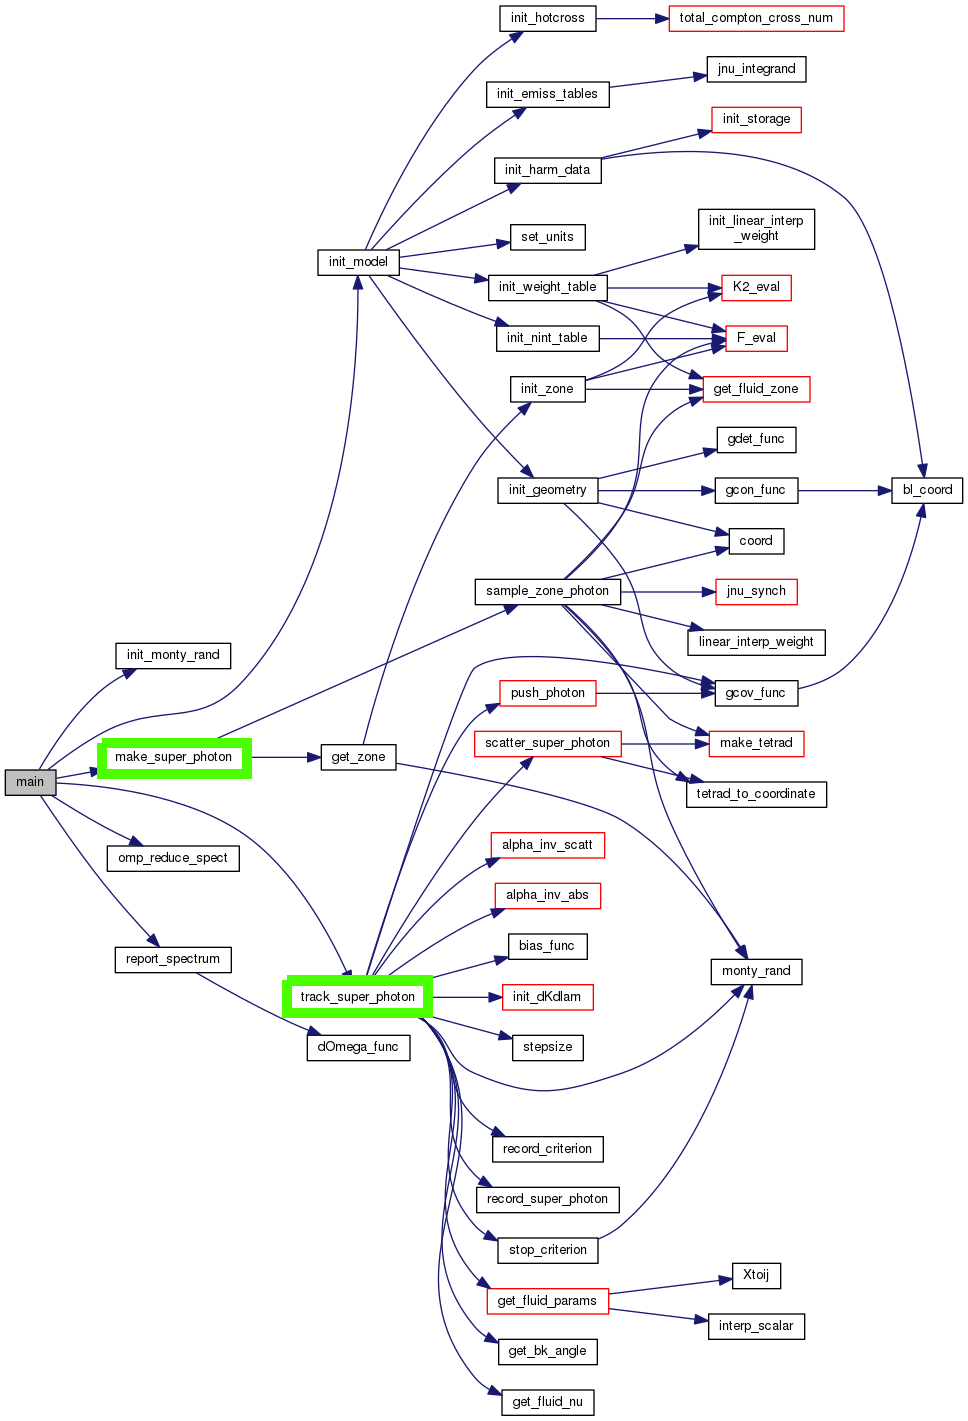
\includegraphics[width=.80\textwidth]{grmonty_graph.png}
    \caption{Grafo de chamadas de funções do grmonty, com ênfase em verde para a track e a make super photon}
    \label{fig:grmontyGraph}
  \end{figure}


  Dada a arquitetura do projeto, o foco principal para aumentar a performance é tornar a paralelização feita em OpenMP para CUDA. Para isso se faz necessário que todo o código previamente distribuído pelas threads do OpenMP tornem-se Kernels, funções device, funções que executam exclusivamente na GPGPU. As principais funções do grmonty que são feitas sob o OpenMP são a \textit{make\_super\_photon} e a \textit{track\_super\_photon} que possuem as responsabilidades de gerar um photon e rastrear a sua trajetória até o final, uma delas é também a função que demanda mais processamento. Para um N razoável capaz de gerar dados consistentes e interessantes 96,95\% do tempo de execução é na função \textit{track\_super\_photon} e sendo executada na ordem de cetenas de milhares de vezes, tornando essa função a mais interessante para ser massivamente paralelizada.

\section{Melhorias e Modificações}
  \subsection{OpenMP e Concorrência}
    O grmonty foi originalmente desenvolvido com OpenMP para maximar a paralelização, fazendo com que cada chamada a \textit{make\_super\_photon} e \textit{track\_super\_photon} fosse executada em paralelo e cada dupla de chamadas as duas funções rodaria em cada thread, isto só é possível porque cada fóton pode ser processado de maneira independente. Cada thread que cria e depois traça a trajetória das partículas é independente, porém ainda usam e consultam variáveis globais definidas no modelo criado na inicialização.

    Entretanto o processamento de cada thread, de cada fóton, pode ou não resultar na coleta final de um mais um fóton, para a verificar o ponto de parada do algoritmo se faz necessário que cada thread ao terminar, informe se obteve sucesso ou não e se obteve persistir os dados de seus resultados para análise posterior. Assim existe um ponto no código onde todas as threads tem que parar e esperar, enquanto uma delas acrescenta o valor total de partículas coletadas e armazena os seus dados. Esta tarefa é relativamente simples em OpenMP, como o código a baixo demonstra. Dois sinalizadores para o compilador fazem com que um trecho de código rode como em uma região crítica, uma região onde somente uma thread pode entrar por vez:

    \begin{lstlisting}
void record_super_photon(struct of_photon *ph)
{
  /* inicializacao e verificacoes */
  /* codigo codigo codigo...      */

#pragma omp critical (MAXTAU)
  {
    /* max_tau_scatt eh variavel global externa*/
    if (ph->tau_scatt > max_tau_scatt)
      max_tau_scatt = ph->tau_scatt;
  }

  /* define em qual posicao salvar os dados */
  /* codigo codigo codigo codigo codigo...  */

#pragma omp atomic
  N_superph_recorded++; /* incrementa o numero fotons coletados */
#pragma omp atomic
  N_scatt += ph->nscatt;

  /* salva os dados */
  /* codigo...      */
}
    \end{lstlisting}

    É possível observar no código acima as directivas do OpenMP, as quais são responsáveis por assegurar que o código definido sob elas irá ser executado por apenas uma thread por vez, nunca duas ao mesmo tempo. Nota-se também que são usadas duas diretivas diferentes, a \textit{\#pragma omp atomic} e a \textit{\#pragma omp critical (<TAG>) } (onde <TAG> pode ser um nome qualquer), Essas diretivas tem uma função muito especial e difícil de ser reproduzida em CUDA.

    A biblioteca OpenMP possui algumas diretivas especificas que informam o compilador certas regras ao gerar código, as duas vistas a cima tem essa função. A \textit{\#pragma omp atomic} é a mais simples, ela tem o objetivo de informar o compilador que o trecho de código logo a baixo dela deve ser tratado como algo atômico, em outras palavras, que deve ser feito de uma única vez, não sendo permitido uma troca de contexto enquanto uma thread está sob essa diretiva. O outro pragma é um pouco mais complexo, é o \textit{\#pragma omp critical (<TAG>) }, é possível  dizer que funciona como o anterior porém com algumas diferença. A primeira é a TAG, essa etiqueta é um nome qualquer escolhido pelo programador para identificar aquela região crítica de outras existentes no código. Enquanto o \textit{omp atomic} para toda e qualquer thread de atuar, o \textit{omp critical} somente vai impedir que outras threads no mesmo bloco identificado executem, isso lhe trás duas vantagens que a outra diretiva não tem: códigos mais complexos podem ser executados, algo que não é permitido no \textit{omp atomic}, e o código lá executado não necessariamente vai bloquear toda a aplicação.

    Essas diretivas do OpenMP funcionam por que são baseadas na POSIX threads api (POSIX), uma interface onde podem ser feitas chamadas ao sistema operacional e programas vão ser executados respeitando o padrão POSIX prestabelecido. Assim, já é conhecida e a muito tempo divulgada a interface com o CPU no que diz respeito programação multithread, porém no universo das GPGPUs esses padrões não existem ou são muito novos.

    Em CUDA a duas diretivas que o OpenMP faz podem ser implementadas, mas com uma dificuldade a mais. O \textit{\#pragma omp atomic} quanto utilizado para a soma, como no código a cima na linha 16 e 17 pode ser feito com a função CUDA \textit{atomicAdd} onde é possivel realizar uma soma em uma thread de forma atômica, sem que ocorra alguma condição de corrida entre as threads sendo possível atualizar o valor sem grandes problemas.

    A implementação já se complica quando tentamos transcrever a parte do código da região crítica. O bloco em questão é o das linhas 6 a 11, nele existem duas ações de resolução complicada, o condicional e a atribuição.

    A atribuição infelizmente não poderia ser implementada por um \textit{atômicas} como nas linhas 16 e 17, pois mesmo não sendo uma soma poderíamos escrever como se fosse. O trecho:
    \begin{lstlisting}
      max_tau_scatt = ph->tau_scatt;
    \end{lstlisting}

    poderia ser reescrito como:

    \begin{lstlisting}
      max_tau_scatt += (- max_tau_scatt + ph->tau_scatt);
    \end{lstlisting}

    mas ainda assim não funcionaria pois o \textit{atomicAdd} só realiza uma adição de forma atômica e a segunda forma precisa de duas adições e as duas tem quer ser feitas de uma vez. Isso é devido ao fato que ao se calcular o que deve ser adicionado a \textit{max\_tau\_scatt} utiliza-se o próprio \textit{max\_tau\_scatt} assim, é possível que o seu valor seja alterado por alguma outra thread entre o cálculo do o que deve ser adicionado e finalmente ser adicionado.

    Este dado já suficiente para descartamos o \textit{atomicAdd}, porém implementar uma região crítica a esse nível na GPGPU não é uma tarefa trivial, e devemos implementar um condicional também. Existem formas de criar regiões criticas na GPGPUs, como por exemplo o \textit{atomicCAS} que realiza uma comparação e dependendo do resultado faz uma atribuição ou não, tudo isso de forma atômica.

    Mas as threads em uma GPGPU não são independentes como as threads da CPU. As threads das GPGPUs e GPUs são agrupadas em grupos de 32, normalmente chamados de \textit{warps}. Todas as threads em um mesmo warp executam as instruções em uma forma completamente \textit{lock-step}, isto é, cada step que uma thread anda todas as outras também andam ao mesmo tempo. Se uma preposição de controle como um condicional ou um laço resulta em alguma ou algumas das 32 threads divergirem do resto, as threads remanescentes vão ficar em espera, dormindo, até as outras terminarem \citep{bestparccuda}.

    No caso de implementar a região crítica utilizando o \textit{atomicCAS} para criar um mutex, deixaria algumas threads passarem enquanto outras ficariam esperando o mutex por um tempo indeterminado, uma vez que não há nada que reforce uma justiça fraca no escalonamento das threads da GPU, resultando num programa que nunca terminaria, entrando em deadlock.

    Uma forma de resolver esse problema é permitindo que cada thread salve em um vetor compartilhado o valor de seu \textit{ph->tau\_scatt}, depois disso somente uma thread é encarregada de achar o maior valor e atribuir esse valor a \textit{max\_tau\_scatt}. A implementação dessa resolução está a baixo:

    \begin{lstlisting}
void record_super_photon(struct of_photon *ph)
{
  /* inicializacao e verificacoes */
  /* codigo codigo codigo...      */

  my_max_tau[thread_uniq_id] = ph->tau_scatt

  __syncthreads();

  if( thread_uniq_id == 0 ) /* somente uma das threads executa esse bloco */
    for(size_t i = 0; i < max_threads; i++){
      if(max_tau_scatt < my_max_tau[i])
        max_tau_scatt = my_max_tau[i]

  __syncthreads();

  /* define em qual posicao salvar os dados */
  /* codigo codigo codigo codigo codigo...  */

  atomicAdd(&N_superph_recorded, 1);
  atomicAdd(&N_scatt, ph->nscatt);

  /* salva os dados */
  /* codigo...      */
}
    \end{lstlisting}

    A biblioteca OpenMP trouxe grande potência e simplicidade para o código do grmonty, mas ao se utilizar a programação em GPGPUs como CUDA, usar em conjunto essa biblioteca pode não ser somente mais complcado como prejudicial a aplicação.

    Diferentemente da possibilidade de sempre ser possível criar um processo novo e lançá-lo a CPU, isso nem sempre é possível na GPU, na realidade o lançamento de diversos kernels a GPGPU sem que ela tenha terminado um antes de vir o outro, pode tornar todo o processamento mais lento ou matar a aplicação que estava sendo executada anteriormente. Por motivos como esses não é uma boa prática tentar lançar vários kernel atraves do OpenMP.

    Como o OpenMP é amplamente usado no grmonty, porém somente em algumas áreas específicas seria interessante usar a programação em GPGPU, o código OpenMP continua presente em algumas partes da aplicação. Os trecho de código mais computacionalmente pesados e com potencial para a a paralelização nestes sim é retirada a integração com o OpenMP e o código é portado para CUDA.

    Analisando o gráfico de processamento com indicação de performance, a figura \ref{fig:grmonty-performance} é evidente que o gargalo da aplicação é a função \textit{track\_super\_photon}. Por é que ela foi a escolhida para ser portada para a GPGPU, além de poder ser altamente paralelizável.

    \begin{figure}[!h]
      \centering
      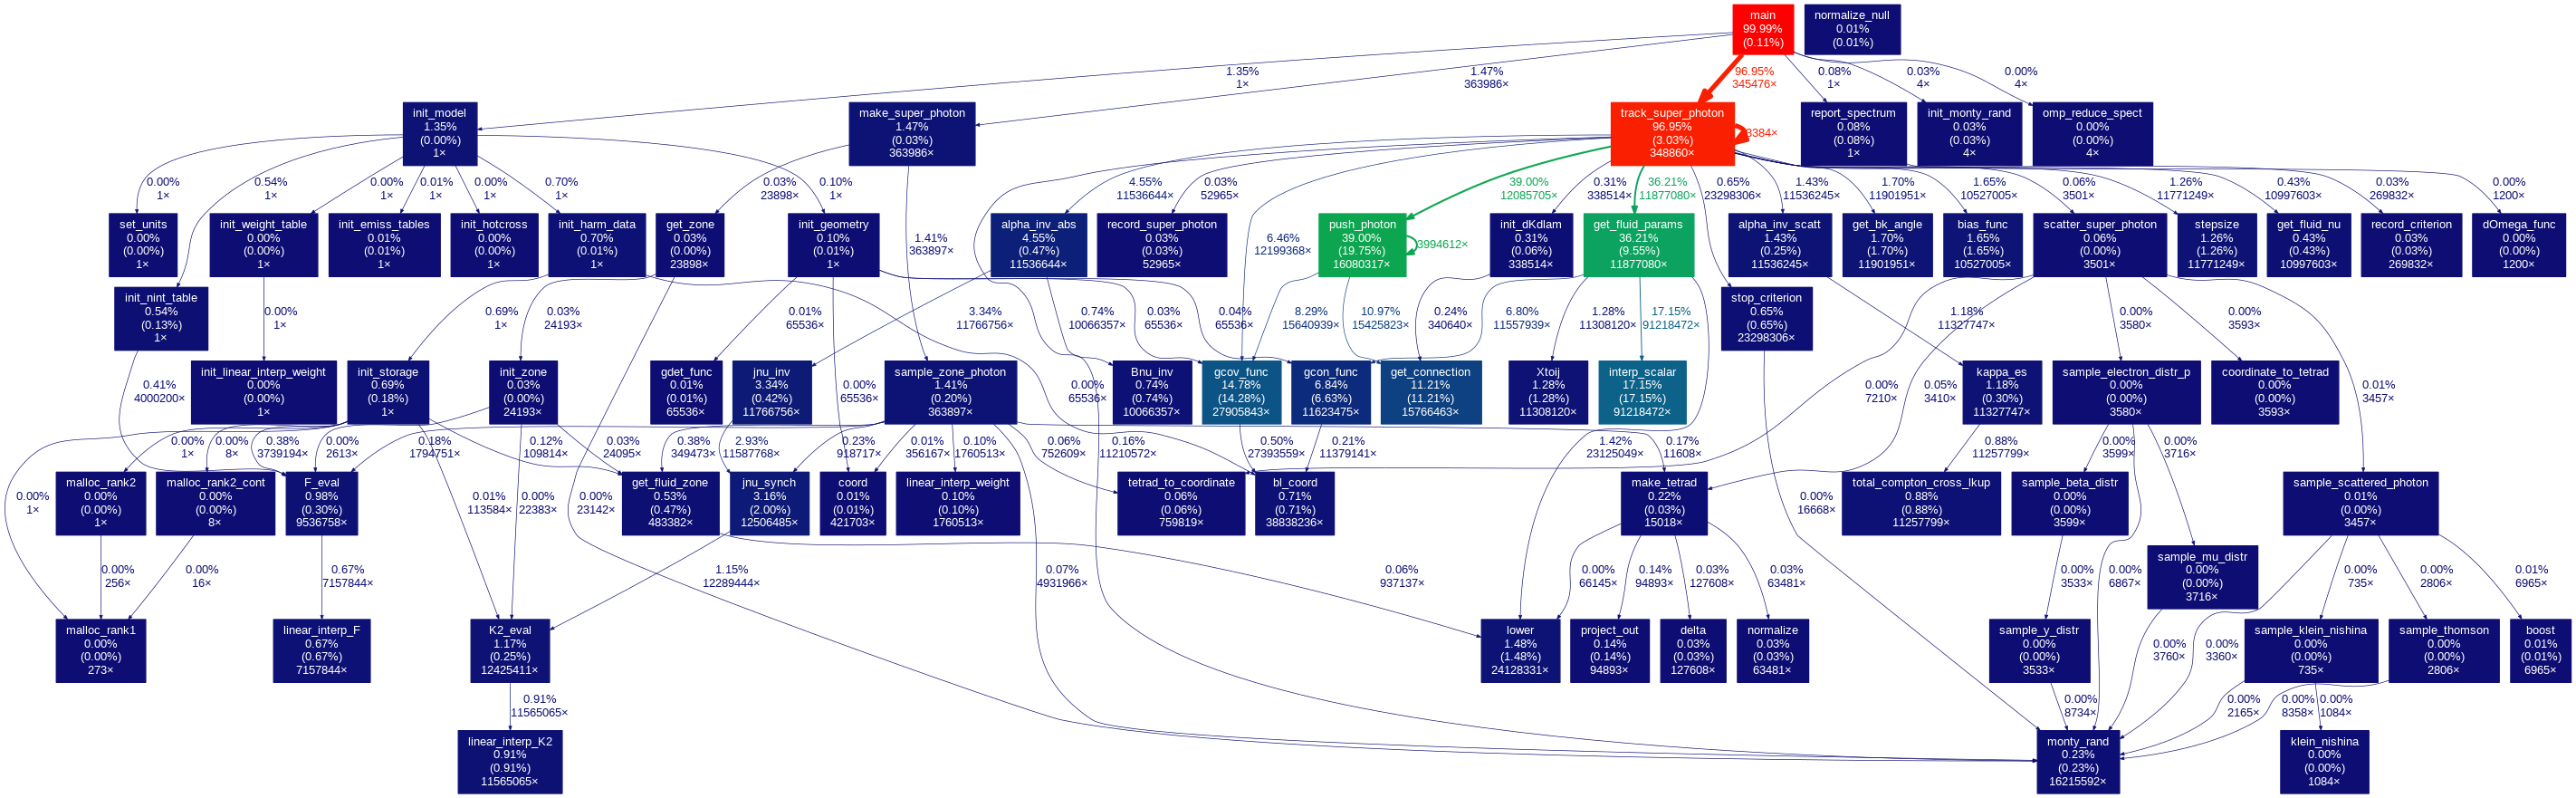
\includegraphics[width=1\textwidth]{time_per_func.png}
      \caption{grafo de funcionamento do grmonty. Quanto mais vermelho mais tempo foi gasto. executados em um Ubuntu 17.10, x64, AMD Fx-6100 six-core processor, 8gb de ram. porcentagem tempo gasto até o retorno da função, porcentagem em parêntesis é o tempo gasto somente dentro da função, não contando outras chamadas.}
      \label{fig:grmonty-performance}
    \end{figure}

  \subsection{funções matemáticas}
    Algumas funções matemáticas que o grmonty usa e que são implementadas pela gnu scientific library (gsl) não podem ser executadas na GPU uma vez que não existe suporte para essa biblioteca pela a Nvidia, porém existe uma biblioteca similar da própria nvidia, a CUDAmath que apresenta uma grande coleção de funções matemáticas que podem servir como substitutas as da gsl.

    O grmonty utiliza as funções:
    \begin{itemize}
      \item \textit{int gsl\_sf\_bessel\_Kn\_e(int n, double x, gsl\_sf\_result * result)} método de calcula a função de Bessel cilindrica modificada irregular de ordem n no ponto x
      \item \textit{void gsl\_ran\_dir\_3d(const gsl\_rng * r, double * x, double * y, double * z)} Função que retorna um vetor normal de três dimensões aleatório com distribuição uniforme.
      \item \textit{double gsl\_rng\_uniform(const gsl\_rng * r)} Função que devolve um número aleatório de precisão dupla entre os valores de 0 e 1, excluindo ambos.
    \end{itemize}

    Destas a primeira e a última possuem uma função equivalente na biblioteca CUDAmath. Só existe uma ressalva sobre a primeira função, pois a gsl funciona para qualquer ordem N, enquanto a implementada pela cuda é somente para as ordens 0 e 1. Felizmente no processamento do track super photon somente a de ordem 1 é necessária.

    A segunda função \textit{void gsl\_ran\_dir\_3d(const gsl\_rng * r, double * x, double * y, double * z)} não contém uma equivalente em CUDAmath, por isso ela teve que ser implementa durante o desenvolvimento do código CUDA.


  \subsection{divisão e trabalho e paralelização}
    O grmonty paraleliza sua carga de trabalho via OpenMP, desta forma o programa tem total acesso a memoria RAM e aos núcleos do processador. Todo o escalonamento de memória e processamento é administrado pelo sistema operacional. A partir do momento que o código passa a ser executado na GPGPU esse controle fino não tem como ser mais terceirizado ao sistema operacional, é de responsabilidade do programador administrar a memória e threads na GPGPU.

    A GPGPU utilizada nos testes é uma Nvida Geforce GTX 550TI, com 192 núcleos e 1024 Mb de memória. Para ser possível utilizar o máximo desse aparelho é necessário mandar cargas de trabalho que utilizem todos os recursos na capacidade mais próxima a da máxima. Ao se utilizar, por exemplo uma carga de tralho de 1100 Mbs em um primeiro passo de execução usaria 100\% da memória porém na próxima usaria cerca de 10\% da memória disponível, tornando 90\% da memória ociosa, logo desperdiçando recursos. A mesma lógica pode ser aplicada aos núcleos da GPGPU, deve-se priorizar por dividir o número de threads que se deseja rodar por um múltiplo de 192, caso a diferença seja muito grande, ou seja a divisão possua um resto significativo, porém longe de 192, faz com que grande parte do núcleos fiquem ociosos, desta forma desperdiçando recursos e tempo para realizar a alocação que não foi usada.

    Essa peculiaridade da programação em GPUs torna cada programa responsável por se reconfigurar a cada computador novo ao qual se pretende executá-lo, porém é possível programar a alocação de recursos para que sempre seja a melhor possível.

    Existe uma API na tecnologia CUDA que permite a busca por parâmetros dos dispositivos disponíveis para o processamento, assim todo o programa antes de lançar seus kernels pode buscar por informações do sistema em que está sendo executado e confugira-se para otimizar o uso de recursos. por exemplo, para o uso otimizado do núcleos das GPGPUs é feita uma conta simples pra distribuir as threads em blocos na grid de execução das threads.

    Quando se determina o número de threads necessárias para a execução ótima, deve-se dividir este número pela quantidade de blocos que se deseja executar e em quantas threads deve ter cada bloco.

    Os núcleos das GPGPUs são divididas em uma \textit{grid} e está grid é composta por blocos, cada um com uma quantidade de threads. Estes valores - de threads por bloco e número de blocos - são escolhidos no momento de se lança o kernel e podem ter valores dinâmicos. Neste momento queremos dividir o número N de processos nessa arquitetura, onde o nosso objetivo é minimizar o número de threads ociosas. Cada bloco pode alocar somente uma potência de 2. Por exemplo, pode-se alocar 2, 8, 1024 ou 512 threads em um bloco mas não 300, 20 ou 1000, somente números que são potências de 2. A mesma regra vale para a quantidade de blocos, assim devemos encontrar o número de blocos $ x = 2^k $ e a quantidade de threads por bloco $ y = 2^p $ encontrando a solução mais aproximada possível para $$ N = 2^k  * 2^p $$


  \subsection{Processar em Lotes}
    Uma mudança muito importante que deve ser feita para tornar possível a paralelização na GPU e torná-la mais eficiente é mudando o modo de operação do grmonty. Atualmente ele cria um fóton para o rastreio, é uma relação de um pra um, onde não há persistência do fóton, ou acumulo de fótons para a partir disto serem processados.

    No modelo de GPGPU uma mudança para a maior performance seria trocar este modelo de processamento. Permitindo que ele possa ocorrer em forma de batchs (lotes de dados), isto é, um conjunto de fótons é produzido e armazenado para, somente no momento que se chegasse ao tamanho ótimo para ser executado na GPGPU, o kernel ser lançado. Para esta modificação se faz necessário armazenar inicialmente uma grande quantidade de fótons, executando o \textit{make\_super\_photon} diversas vezes até que se consiga um tamanho ótimo para ocupar a GPU e que também faça o processamento ser eficiente na GPGPU.
